%!TEX root = ../final_report.tex

While exploring the environment and discovering objects, the system needs to store a volumetric 3D representation of what it has discovered.
While this could be done by simply dividing the environment into a regular grid of voxels and storing information at each voxel, this is not an efficient way to store spatial information.
Often large subvolumes within the space are required to have the same information -- such as an object candidate label or a label for empty space -- at each of their constituent voxels, and explicitly representing and storing information at each voxel means the same information is stored many times.

One way of improving the efficiency of a volumetric representation is by using an octree\cite{meagher1982octrees}.
Octrees are an extension of the quadtree principle into 3D: at the top level sits a single root node, which represents the entire space to be mapped.
At the next level are eight nodes, each representing one eighth (octant) of the original cube.
This subdivision into eights recurses until the required level of granularity is reached (see figure \ref{fig:octree}).
Because each branch of the tree can be arbitrarily deep, information about a large volume of space can be stored once in a single high level tree node, rather than thousands of times in lowest-level voxels.
In areas where finer granularity is needed, the tree is deepened as required.
Thus the representation can be very fine-grained in areas where it needs to be, and much coarser-grained where such detail is not required.
% In theory an octree can be infinitely deep, although concrete implementations often place limits on the maximum tree depth.

\begin{figure}[ht]
	\begin{center}
		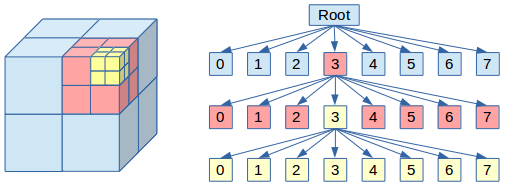
\includegraphics[width=0.6\linewidth]{src/octree.png} 
		\caption[Using an octree to represent a 3D volume]{Using an octree to represent a 3D volume.\footnotemark}
		\label{fig:octree}
	\end{center}
\end{figure}
\footnotetext{{\url{https://geidav.wordpress.com/2014/07/18/advanced-octrees-1- preliminaries-insertion-strategies-and-max-tree-depth}}}